% questions.tex —— 2015 年·陕西卷·文史类 · 题目内容片段（无答案）
% 由 tools/generate_projects.py 依来源总账自 2015/2015_数学真题_陕西文_试题.md 生成，勿手改（改源 MD 后重跑）


\begin{gktip}
来源说明：固定源 2 页 A3，印刷页 975–976，卷内无答案；卷首无注意事项框、无「第Ⅰ卷」字样。Q8 选项 (C) 印作 $(\boldsymbol{a}+\boldsymbol{b})^{2}=|\boldsymbol{a}+\boldsymbol{b}|^{2}$，Q2 饼图每幅只标一个百分数，Q11 表格首列表头空白，均照录未补。

图形说明：第 2、5、7、14、18、20、22 题图依原页拓扑重绘，不按比例；Q11/Q19 表格以 Markdown 表格照录。
\end{gktip}

\begin{gktip}
卷面抬头：2015 普通高等学校招生考试（陕西卷文）

（源疑点：扫描件卷首只有上述标题行，其后直接为「一、选择题」；未见注意事项说明框，卷面也没有「第Ⅰ卷」「第Ⅱ卷」字样。两页页脚印刷页码分别为 975、976，第 976 页直接从第 19 题续排，无页眉。此处照扫描页记录，未按常见卷式补写。）

（源疑点：第 8 题选项 (C) 在扫描页上印作 $(\boldsymbol{a}+\boldsymbol{b})^{2}=|\boldsymbol{a}+\boldsymbol{b}|^{2}$，与常见的 $(\boldsymbol{a}+\boldsymbol{b})^{2}=\boldsymbol{a}^{2}+2\boldsymbol{a}\cdot\boldsymbol{b}+\boldsymbol{b}^{2}$ 写法不同；此处照录，未改。）

（源疑点：第 11 题表格首列表头为空白，仅第二、三、四列标「甲」「乙」「原料限额」；此处按原样留空。）

（源疑点：第 2 题右图只标「60\%」与「男」，左图只标「70\%」与「女」，另一扇区未标百分数；此处照录，未补算。）

（源疑点：第 18 题图 2 中，$E$ 为底面顶点，虚线 $A_{1}E$、$OE$、$ED$ 交于 $E$；原扫描页「$E$」字紧贴 $A_{1}C$，易误读为 $E$ 在 $A_{1}C$ 上，重绘按真实拓扑处理。）
\end{gktip}

\gkpart{一、选择题}

\begin{question}
\gkti{1}设集合 $M=\{x\mid x^{2}=x\}$，$N=\{x\mid \lg x\le 0\}$，则 $M\cup N=$（　）。

（A）$[0,1]$；（B）$(0,1]$；（C）$[0,1)$；（D）$(-\infty,1]$。

\Needspace{0.4\textheight}
\end{question}
\begin{question}
\gkti{2}某中学初中部共有 $110$ 名教师，高中部共有 $150$ 名教师，其性别比例如图所示，则该校女教师的人数为（　）。
\nopagebreak[4]
\begin{center}% 2015 年陕西卷（文史类）第 2 题：教师性别比例饼图（依固定扫描页重绘，只画拓扑与标号，不按比例）
\begin{tikzpicture}[scale=1.0]
  % 左图：初中部，女 70%
  \fill[gray!30] (0,0) -- (35:1.3) arc (35:287:1.3) -- cycle;
  \draw (0,0) circle (1.3);
  \draw (0,0) -- (35:1.3);
  \draw (0,0) -- (287:1.3);
  \node at (170:0.72) {70\%};
  \node at (215:0.72) {女};
  \node at (-10:0.62) {男};
  \node at (0,-1.72) {（初中部）};
  % 右图：高中部，男 60%
  \begin{scope}[xshift=4.2cm]
    \fill[gray!30] (0,0) -- (105:1.3) arc (105:249:1.3) -- cycle;
    \draw (0,0) circle (1.3);
    \draw (0,0) -- (105:1.3);
    \draw (0,0) -- (249:1.3);
    \node at (177:0.72) {女};
    \node at (30:0.90) {60\%};
    \node at (-35:0.55) {男};
    \node at (0,-1.72) {（高中部）};
  \end{scope}
\end{tikzpicture}
\end{center}
\nopagebreak[4]
（A）$93$；（B）$123$；（C）$137$；（D）$167$。

\end{question}
\begin{question}
\gkti{3}已知抛物线 $y^{2}=2px$（$p>0$）的准线经过点 $(-1,1)$，则该抛物线焦点坐标为（　）。

（A）$(-1,0)$；（B）$(1,0)$；（C）$(0,-1)$；（D）$(0,1)$。

\end{question}
\begin{question}
\gkti{4}设 $f(x)=\begin{cases}1-\sqrt{x}, & x\ge 0,\\[2pt] 2^{x}, & x<0,\end{cases}$ 则 $f(f(-2))=$（　）。

（A）$-1$；（B）$\dfrac{1}{4}$；（C）$\dfrac{1}{2}$；（D）$\dfrac{3}{2}$。

\Needspace{0.4\textheight}
\end{question}
\begin{question}
\gkti{5}一个几何体的三视图如图所示，则该几何体的表面积为（　）。
\nopagebreak[4]
\begin{center}% 2015 年陕西卷（文史类）第 5 题：三视图（依固定扫描页重绘，只画拓扑与标号，不按比例）
\begin{tikzpicture}[>=stealth,scale=1.0]
  % 正视图：边长 2 的正方形
  \draw (0,0) rectangle (2,2);
  \draw[<->] (0,-0.3)--(2,-0.3);
  \node at (1,-0.62) {$2$};
  \draw[<->] (2.3,0)--(2.3,2);
  \node at (2.68,1) {$2$};
  \node at (1,-1.05) {正视图};
  % 左视图：宽 1、高 2 的长方形（扫描页未标尺寸）
  \draw (4.0,0) rectangle (5.0,2);
  \node at (4.5,-1.05) {左视图};
  % 俯视图：宽 2、高 1 的半圆
  \draw (0,-2.4)--(2,-2.4);
  \draw (0,-2.4) arc (180:0:1);
  \draw[<->] (2.3,-2.4)--(2.3,-1.4);
  \node at (2.68,-1.9) {$1$};
  \node at (1,-3.9) {俯视图};
\end{tikzpicture}
\end{center}
\nopagebreak[4]
（A）$3\pi$；（B）$4\pi$；（C）$2\pi+4$；（D）$3\pi+4$。

\end{question}
\begin{question}
\gkti{6}“$\sin\alpha=\cos\alpha$”是“$\cos 2\alpha=0$”的（　）。

（A）充分不必要条件；（B）必要不充分条件；（C）充分必要条件；（D）既不充分也不必要条件。

\Needspace{0.4\textheight}
\end{question}
\begin{question}
\gkti{7}根据框图，当输入 $x$ 为 $6$ 时，输出的 $y=$（　）。
\nopagebreak[4]
\begin{center}% 2015 年陕西卷（文史类）第 7 题：程序框图（依固定扫描页重绘，只画拓扑与标号，不按比例）
\begin{tikzpicture}[>=stealth,scale=0.95]
  % 开始
  \draw[rounded corners=6pt] (-1.0,0.4) rectangle (1.0,-0.4);
  \node at (0,0) {开始};
  \draw[->] (0,-0.4)--(0,-1.0);
  % 输入 x
  \draw (-1.0,-1.0)--(1.2,-1.0)--(1.0,-1.8)--(-1.2,-1.8)--cycle;
  \node at (0,-1.4) {输入 $x$};
  \draw[->] (0,-1.8)--(0,-2.3);
  % 赋值 x = x - 3
  \draw (-1.3,-2.3) rectangle (1.3,-3.1);
  \node at (0,-2.7) {$x=x-3$};
  \draw[->] (0,-3.1)--(0,-3.7);
  % 判断 x >= 0
  \draw (-1.9,-4.4)--(0,-3.7)--(1.9,-4.4)--(0,-5.1)--cycle;
  \node at (0,-4.4) {$x\ge 0$};
  % 是：回到赋值框
  \draw[->] (1.9,-4.4)--(3.2,-4.4)--(3.2,-2.7)--(1.3,-2.7);
  \node at (2.35,-4.05) {是};
  % 否：向下
  \draw[->] (0,-5.1)--(0,-5.7);
  \node at (0.32,-5.4) {否};
  % y = x^2 + 1
  \draw (-1.4,-5.7) rectangle (1.4,-6.5);
  \node at (0,-6.1) {$y=x^{2}+1$};
  \draw[->] (0,-6.5)--(0,-7.1);
  % 输出 y
  \draw (-1.0,-7.1)--(1.2,-7.1)--(1.0,-7.9)--(-1.2,-7.9)--cycle;
  \node at (0,-7.5) {输出 $y$};
  \draw[->] (0,-7.9)--(0,-8.5);
  % 结束
  \draw[rounded corners=6pt] (-1.0,-8.5) rectangle (1.0,-9.3);
  \node at (0,-8.9) {结束};
\end{tikzpicture}
\end{center}
\nopagebreak[4]
（A）$1$；（B）$2$；（C）$5$；（D）$10$。

\end{question}
\begin{question}
\gkti{8}对任意向量 $\boldsymbol{a}$，$\boldsymbol{b}$，下列关系式中不恒成立的是（　）。

（A）$|\boldsymbol{a}\cdot\boldsymbol{b}|\le|\boldsymbol{a}||\boldsymbol{b}|$；（B）$|\boldsymbol{a}-\boldsymbol{b}|\le||\boldsymbol{a}|-|\boldsymbol{b}||$；（C）$(\boldsymbol{a}+\boldsymbol{b})^{2}=|\boldsymbol{a}+\boldsymbol{b}|^{2}$；（D）$(\boldsymbol{a}+\boldsymbol{b})\cdot(\boldsymbol{a}-\boldsymbol{b})=\boldsymbol{a}^{2}-\boldsymbol{b}^{2}$。

\end{question}
\begin{question}
\gkti{9}设 $f(x)=x-\sin x$，则 $f(x)$（　）。

（A）既是奇函数又是减函数；（B）既是奇函数又是增函数；（C）是有零点的减函数；（D）是没有零点的奇函数。

\end{question}
\begin{question}
\gkti{10}设 $f(x)=\ln x$，$0<a<b$，若 $p=f\left(\sqrt{ab}\right)$，$q=f\left(\dfrac{a+b}{2}\right)$，$r=\dfrac{1}{2}(f(a)+f(b))$，则下列关系式中正确的是（　）。

（A）$q=r<p$；（B）$q=r>p$；（C）$p=r<q$；（D）$p=r>q$。

\end{question}
\begin{question}
\gkti{11}某企业生产甲、乙两种产品均需用 $A$，$B$ 两种原料，已知生产 $1$ 吨每种产品所需原料及每天原料的可用限额如表所示．如果生产 $1$ 吨甲、乙产品可获利润分别为 $3$ 万元、$4$ 万元，则该企业每天可获得最大利润为（　）。

\begin{center}
\begin{tabular}{llll}
\toprule
 & 甲 & 乙 & 原料限额 \\
\midrule
$A$（吨） & $3$ & $2$ & $12$ \\
$B$（吨） & $1$ & $2$ & $8$ \\
\bottomrule
\end{tabular}
\end{center}

（A）$12$ 万元；（B）$16$ 万元；（C）$17$ 万元；（D）$18$ 万元。

\end{question}
\begin{question}
\gkti{12}设复数 $z=(x-1)+y\mathrm{i}$（$x,y\in\mathbf{R}$），若 $|z|\le 1$，则 $y\ge x$ 的概率为（　）。

（A）$\dfrac{3}{4}+\dfrac{1}{2\pi}$；（B）$\dfrac{1}{2}+\dfrac{1}{\pi}$；（C）$\dfrac{1}{4}-\dfrac{1}{2\pi}$；（D）$\dfrac{1}{2}-\dfrac{1}{\pi}$。

\end{question}
\gkpart{二、填空题}

\begin{question}
\gkti{13}中位数为 $1010$ 的一组数构成等差数列，其末项为 $2015$，则该数列的首项为 \gkblank{}。

\Needspace{0.4\textheight}
\end{question}
\begin{question}
\gkti{14}如图，某港口一天 $6$ 时到 $18$ 时的水深变化曲线近似满足函数 $y=3\sin\left(\dfrac{\pi}{6}x+\varphi\right)+k$．据此函数可知，这段时间水深（单位：$\mathrm{m}$）的最大值为 \gkblank{}。
\nopagebreak[4]
\begin{center}% 2015 年陕西卷（文史类）第 14 题：水深随时间变化的曲线（依固定扫描页重绘，只画拓扑与标号，不按比例）
\begin{tikzpicture}[>=stealth,scale=1.0,xscale=0.55,yscale=0.62]
  % 坐标轴
  \draw[->] (0,0)--(7.2,0) node[above right] {时间/t};
  \draw[->] (0,-0.5)--(0,4.0) node[above right] {水深/m};
  \node[below left] at (0,0) {$O$};
  \node[left] at (0,1.0) {$2$};
  % 最低水位的虚线
  \draw[dashed] (0,1.0)--(2.82,1.0);
  % 曲线：最小值 2，最大值 8（示意）
  \draw[thick,domain=1.9:5.6,samples=120] plot (\x,{2.5-1.5*cos(180*(\x-2.82)/1.85)});
  % 时刻刻度
  \draw (1.9,0.06)--(1.9,-0.06);
  \node[below] at (1.9,0) {$6$};
  \draw (5.6,0.06)--(5.6,-0.06);
  \node[below] at (5.6,0) {$18$};
\end{tikzpicture}
\end{center}
\nopagebreak[4]
\end{question}
\begin{question}
\gkti{15}函数 $y=x\mathrm{e}^{x}$ 在其极值点处的切线方程为 \gkblank{}。

\end{question}
\begin{question}
\gkti{16}观察下列等式：

\nopagebreak[4]
\[
\begin{aligned}
1-\frac{1}{2}&=\frac{1}{2},\\
1-\frac{1}{2}+\frac{1}{3}-\frac{1}{4}&=\frac{1}{3}+\frac{1}{4},\\
1-\frac{1}{2}+\frac{1}{3}-\frac{1}{4}+\frac{1}{5}-\frac{1}{6}&=\frac{1}{4}+\frac{1}{5}+\frac{1}{6},\\
&\cdots\cdots,
\end{aligned}
\]

据此规律，第 $n$ 个等式可为 \gkblank{}。

\end{question}
\gkpart{三、解答题}

\begin{question}
\gkti{17}$\triangle ABC$ 的内角 $A$，$B$，$C$ 所对的边分别为 $a$，$b$，$c$．向量 $\boldsymbol{m}=(a,\sqrt{3}b)$ 与 $\boldsymbol{n}=(\cos A,\sin B)$ 平行．

（1） 求 $A$；

（2） 若 $a=\sqrt{7}$，$b=2$，求 $\triangle ABC$ 的面积．

\Needspace{0.4\textheight}
\end{question}
\begin{question}
\gkti{18}如图 1，在直角梯形 $ABCD$ 中，$AD\parallel BC$，$\angle BAD=\dfrac{\pi}{2}$，$AB=BC=\dfrac{1}{2}AD=a$，$E$ 是 $AD$ 的中点，$O$ 是 $AC$ 与 $BE$ 的交点．将 $\triangle ABE$ 沿 $BE$ 折起到图 2 中 $\triangle A_{1}BE$ 的位置，得到四棱锥 $A_{1}-BCDE$．

（1） 证明：$CD\perp$ 平面 $A_{1}OC$；

（2） 若平面 $A_{1}BE\perp$ 平面 $BCDE$，四棱锥 $A_{1}-BCDE$ 的体积为 $36\sqrt{2}$，求 $a$ 的值．
\nopagebreak[4]
\begin{center}% 2015 年陕西卷（文史类）第 18 题：折叠前的直角梯形与折叠后的四棱锥（依固定扫描页重绘，只画拓扑与标号，不按比例）
\begin{tikzpicture}[scale=0.85]
  % 图 1：直角梯形 ABCD，E 为 AD 中点，O 为 AC 与 BE 的交点
  \coordinate (A) at (0,2);
  \coordinate (B) at (0,0);
  \coordinate (C) at (2,0);
  \coordinate (D) at (3,2);
  \coordinate (E) at (1.5,2);
  \coordinate (O) at (0.75,1.25);
  \draw (A)--(D)--(C)--(B)--cycle;
  \draw (A)--(C);
  \draw (B)--(E);
  \node[above left] at (A) {$A$};
  \node[below left] at (B) {$B$};
  \node[below] at (C) {$C$};
  \node[above right] at (D) {$D$};
  \node[above] at (E) {$E$};
  \node[left] at (O) {$O$};
  \node at (1.5,-0.75) {图 1};
  % 图 2：折叠后所得四棱锥 A1-BCDE
  \begin{scope}[xshift=5.4cm]
    \coordinate (A1) at (0.9,3.0);
    \coordinate (B2) at (0.2,0.2);
    \coordinate (C2) at (2.2,0.2);
    \coordinate (D2) at (3.4,1.4);
    \coordinate (E2) at (1.4,1.4);
    \coordinate (O2) at (0.8,0.8);
    % 可见侧棱与底边：实线
    \draw (A1)--(B2);
    \draw (A1)--(C2);
    \draw (A1)--(D2);
    \draw (B2)--(C2);
    \draw (C2)--(D2);
    % 被遮挡的棱与辅助线：虚线
    \draw[dashed] (A1)--(E2);
    \draw[dashed] (D2)--(E2);
    \draw[dashed] (A1)--(O2);
    \draw[dashed] (B2)--(O2);
    \draw[dashed] (O2)--(E2);
    \draw[dashed] (O2)--(C2);
    \node[above] at (A1) {$A_{1}(A)$};
    \node[below left] at (B2) {$B$};
    \node[below] at (C2) {$C$};
    \node[right] at (D2) {$D$};
    \node[above left] at (E2) {$E$};
    \node[below] at (O2) {$O$};
    \node at (1.7,-0.75) {图 2};
  \end{scope}
\end{tikzpicture}
\end{center}
\nopagebreak[4]
\end{question}
\begin{question}
\gkti{19}随机抽取一个年份，对西安市该年 $4$ 月份的天气情况进行统计，结果如下：

\begin{center}
\begingroup\setlength{\tabcolsep}{4pt}
\begin{tabular}{lllllllllll}
\toprule
日期 & 1 & 2 & 3 & 4 & 5 & 6 & 7 & 8 & 9 & 10 \\
\midrule
天气 & 晴 & 雨 & 阴 & 阴 & 阴 & 雨 & 阴 & 晴 & 晴 & 晴 \\
日期 & 11 & 12 & 13 & 14 & 15 & 16 & 17 & 18 & 19 & 20 \\
天气 & 阴 & 晴 & 晴 & 晴 & 晴 & 晴 & 阴 & 雨 & 阴 & 阴 \\
日期 & 21 & 22 & 23 & 24 & 25 & 26 & 27 & 28 & 29 & 30 \\
天气 & 晴 & 阴 & 晴 & 晴 & 晴 & 阴 & 晴 & 晴 & 晴 & 雨 \\
\bottomrule
\end{tabular}
\endgroup
\end{center}

（1） 在 $4$ 月份任取一天，估计西安市在该天不下雨的概率；

（2） 西安市某学校拟从 $4$ 月份的一个晴天开始举行连续 $2$ 天的运动会，估计运动会期间不下雨的概率．

\Needspace{0.4\textheight}
\end{question}
\begin{question}
\gkti{20}如图，椭圆 $E$：$\dfrac{x^{2}}{a^{2}}+\dfrac{y^{2}}{b^{2}}=1$（$a>b>0$）经过点 $A(0,-1)$，且离心率为 $\dfrac{\sqrt{2}}{2}$．

（1） 求椭圆 $E$ 的方程；

（2） 经过点 $(1,1)$，且斜率为 $k$ 的直线与椭圆 $E$ 交于不同的两点 $P$，$Q$（均异于点 $A$），证明：直线 $AP$ 与 $AQ$ 的斜率之和为 $2$．
\nopagebreak[4]
\begin{center}% 2015 年陕西卷（文史类）第 20 题：椭圆与过定点的弦（依固定扫描页重绘，只画拓扑与标号，不按比例）
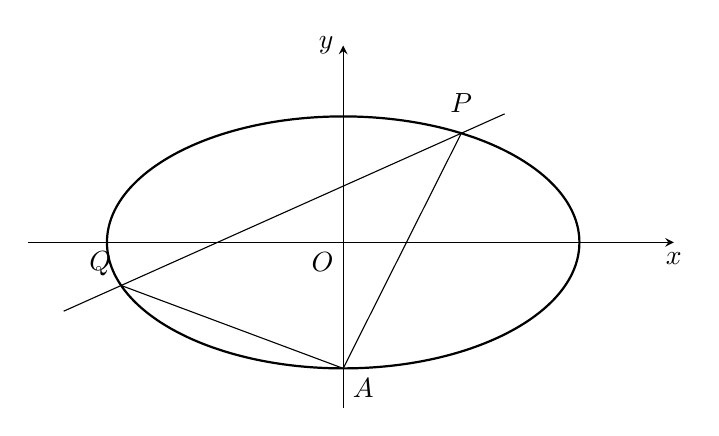
\begin{tikzpicture}[>=stealth,scale=1.0]
  % 坐标轴
  \draw[->] (-4.0,0)--(4.2,0) node[below] {$x$};
  \draw[->] (0,-2.1)--(0,2.5) node[left] {$y$};
  \node[below left] at (0,0) {$O$};
  % 椭圆
  \draw[thick] (0,0) ellipse (3 and 1.6);
  % 点 P、Q 与弦 PQ
  \coordinate (P) at (1.5,1.386);
  \coordinate (Q) at (-2.82,-0.547);
  \coordinate (A) at (0,-1.6);
  \draw (2.05,1.632)--(-3.55,-0.874);
  \draw (A)--(P);
  \draw (A)--(Q);
  \node[above=4pt] at (P) {$P$};
  \node[above left] at (Q) {$Q$};
  \node[below right] at (A) {$A$};
\end{tikzpicture}
\end{center}
\nopagebreak[4]
\end{question}
\begin{question}
\gkti{21}设 $f_{n}(x)=x+x^{2}+\cdots+x^{n}-1$，$x\ge 0$，$n\in\mathbf{N}$，$n\ge 2$．

（1） 求 $f_{n}'(2)$；

（2） 证明：$f_{n}(x)$ 在 $\left(0,\dfrac{2}{3}\right)$ 内有且仅有一个零点（记为 $a_{n}$），且 $0<a_{n}-\dfrac{1}{2}<\dfrac{1}{3}\left(\dfrac{2}{3}\right)^{n}$．

\Needspace{0.4\textheight}
\end{question}
\begin{question}
\gkti{22}如图，$AB$ 切 $\odot O$ 于点 $B$，直线 $AO$ 交 $\odot O$ 于 $D$，$E$ 两点，$BC\perp DE$，垂足为 $C$．

（1） 证明：$\angle CBD=\angle DBA$；

（2） 若 $AD=3DC$，$BC=\sqrt{2}$，求 $\odot O$ 的直径．
\nopagebreak[4]
\begin{center}% 2015 年陕西卷（文史类）第 22 题：圆的切线与割线（依固定扫描页重绘，只画拓扑与标号，不按比例）
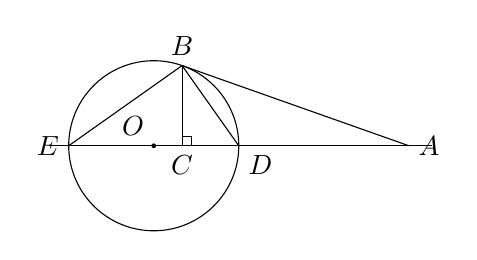
\begin{tikzpicture}[>=stealth,scale=0.72]
  % 圆 O
  \draw (0,0) circle (1.5);
  \fill (0,0) circle (1.2pt);
  \node[above left] at (0,0) {$O$};
  % 割线 A-D-C-O-E
  \draw (-1.85,0)--(4.9,0);
  \coordinate (E) at (-1.5,0);
  \coordinate (C) at (0.5,0);
  \coordinate (D) at (1.5,0);
  \coordinate (A) at (4.5,0);
  \coordinate (B) at (0.5,1.414);
  % 切线与弦
  \draw (B)--(A);
  \draw (B)--(E);
  \draw (B)--(D);
  \draw (B)--(C);
  % 直角标记
  \draw (0.5,0.16)--(0.66,0.16)--(0.66,0);
  % 标号
  \node[above] at (B) {$B$};
  \node[left] at (E) {$E$};
  \node[below] at (C) {$C$};
  \node[below right] at (D) {$D$};
  \node[right] at (A) {$A$};
\end{tikzpicture}
\end{center}
\nopagebreak[4]
\end{question}
\begin{question}
\gkti{23}在直角坐标系 $xOy$ 中，直线 $l$ 的参数方程为 $\begin{cases}x=3+\dfrac{1}{2}t,\\[4pt] y=\dfrac{\sqrt{3}}{2}t,\end{cases}$（$t$ 为参数），以原点为极点，$x$ 轴正半轴为极轴建立极坐标系，$\odot C$ 的极坐标方程为 $\rho=2\sqrt{3}\sin\theta$．

（1） 写出 $\odot C$ 的直角坐标方程；

（2） $P$ 为直线 $l$ 上一动点，当 $P$ 到圆心 $C$ 的距离最小时，求 $P$ 的直角坐标．

\end{question}
\begin{question}
\gkti{24}已知关于 $x$ 的不等式 $|x+a|<b$ 的解集为 $\{x\mid 2<x<4\}$．

（1） 求实数 $a$，$b$ 的值；

（2） 求 $\sqrt{at+12}+\sqrt{bt}$ 的最大值．

\end{question}